\chapter{Design}
In this chapter we will discuss the architecture of the prototype.
It's divided into two section: Dataset and Model. Since
the dataset is standalone component, this seems to be
a reasonable separation. To make it clear, dataset would be a component
which holds the training, validation and test data including all relevant
functionality that can or should be performed on the
data(this is explained more detailed in \autoref{sec:design_data}).
Model would be a component, which accepts the data(dataset component), performs
training on the training data, and then makes inference on the test dataset.
In other words, model would be everything what is related to building,
training and evaluation of neural networks and reinforcement learning environment.



\section{Dataset}
\label{sec:design_data}

Dataset is component which is responsible for data holding. It should
accept original MNIST dataset and transform it into dataset described
in \autoref{sec:analysis_dataset}.

\paragraph{MNIST Dataset} is dataset of scanned handwritten images, each labeled
from 0 to 9. You can see an example of 4 digits in figure \ref{fig:mnist}.
Additionally, it includes label for each of the image.

\begin{figure}[h!]
	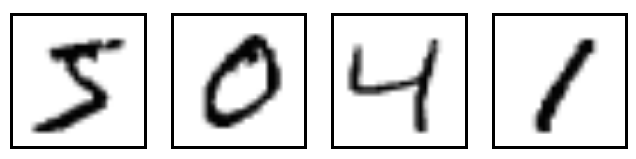
\includegraphics[width=\linewidth,scale=0.4]{MNIST}
	\caption{MNIST example}
	\label{fig:mnist}
\end{figure}

For example, in the figure \ref{fig:mnist} the labels are 5, 0, 4 and 1.

TensorFlow provides a small class \lstinline{Dataset}\footnote{
The class is implemented here: https://github.com/tensorflow/tensorflow/blob/master/tensorflow/contrib/learn/python/learn/datasets/mnist.py
} which stores MNIST data and splits it into training,
validation and test data. TensorFlow also provides functions for iterating
over the batches.
TensorFlow also provides the function which downloads and read the original data
from MNIST web site. Taking this into account, in this work we will abstract from
downloading and reading MNIST data by using this class. We'll refer
to this as \emph{MNIST tf-dataset class}

Remove this:
\begin{lstlisting}[language=Python]
from tensorflow.examples.tutorials.mnist import input_data
mnist = input_data.read_data_sets("MNIST_data/", one_hot=True)
\end{lstlisting}
This two lines will download the data and store into "MNIST_data/" directory.

It is common knowledge that google take a special care about the quality of their code,
therefore our dataset component should have the similar
behaviour and functionality as MNIST tf-dataset class. Another reason for that
is that we want to stay consistent with tensorFlow practices as we use this library
in this work.

% Dataset is a non-real world data, but may behave and represent similar
% task as it could in real world data.
% \paragraph{explain original MNIST data, what is there, how does this work,
% and tf class is used to provide the utility}

% \paragraph{Obstacles} Using the procedure described in \autoref{sec:design_data}
% to create the dataset several obstacles can arise.
% we need to make sure that no same non-noise picture come up with in the dataset.

% To make the dataset
% By build the dataset, we need to consider following
To make dataset free of any dependencies, we need to make sure that two
same noise wouldn't come up more then once in the one of the classes.
Therefore we need 
% we want the model to generalise on unseen data.
Dataset component should be flexible enough in order to be similar to real problem,
therefore to be able to experiment with different amount of classes, and
different variations of noises classes. component should be
 At that point we don't know how the model will behave



\paragraph{Requirements} Like why do we need index generator
including flexibility
\paragraph{Inspiration fromt the tf class dataset}

inpsiration from dataset class from tensor flow: link
% https://github.com/tensorflow/tensorflow/blob/master/tensorflow/contrib/learn/python/learn/datasets/mnist.py
that should perform similar action to
% The function requirement to the dataset can be formulated as

\paragraph{
	not learning any dependency,
	explain that we want to avoid the same samples in a group to avoid that
}
% model will learn dependency and etc.

\paragraph{
	explain shortly about combinations of MNIST data, how to achieve the best data
}

\paragraph{then show the uml diagram of dataset}
including: Class overview

\paragraph{explain what is purpose of each of the class. }

\paragraph{explain what design pattern was applied on that with reference to
the Analysis.}

inderect variable access. (e.g.)

\section{Model}
\label{sec:design_model}

\paragraph{Why did you choose picker network?}
\paragraph{about why OO programming is not ALMOST suited and why it should be more functional}
\paragraph{The architecture as a whole}
\paragraph{Possbile classes, overview}
\paragraph{UML diagram}
\paragraph{back up the classes with design patterns}

\paragraph{the flow of the data via function}


\subsection{Configuration of the project, what can be configured, the complexity of the model}





the curent desing is using the approach
described in \autoref{ssec:picker_net}.

Basically explain the flow of input data, all losses, and baselines, and etc.
if there is anything relative to the structure in the code use the references to the design patters
Show all classes, write the documentation for those, or at least briefly explain the purpose.
The process of training, maybe explain the whole idea behind this
	seperation of dataset into validation, test, training.
look at the other bachelorarbeits and look of what they wrote there
think about whether it's possible to combine the design and implemntation chapters



* Entwurfsstrategie, Beschreibungen funktionaler und nich
 funktionaler Anforderungen, Einsatz von Mustern und
 Bibliotheken, Softwarearchitektur, Verwendung von Datentypen und
 Datenstrukturen, Algorithmen, Mensch-Maschine-Schnittstelle;
